%! Author = Sujal Singh
%! Date = 10/18/23

% Preamble
%! suppress = FileNotFound
\documentclass[11pt]{ipu-c}
\usepackage[
    pdftitle={C Programming Lab Practical File},
    pdfsubject={C Programming Lab Practical File},
    pdfauthor={Sujal Singh},
    pdfdisplaydoctitle,
    hidelinks,
]{hyperref}

% Packages
\usepackage{amsmath}
\usepackage[indLines]{algpseudocodex}

% Document
\begin{document}
    \maketitle

    %----------------------------------------------------- Index ------------------------------------------------------%
    % Doing this manually for now because I don't have the time/will to automate it, should've been a simple enough    %
    % thing but from a few searches on the web, it doesn't seem that easy.                                             %
    %------------------------------------------------------------------------------------------------------------------%

    \newpage
    \pagenumbering{gobble}
    \begin{center}
        \textbf{\Huge Index} \\[20pt]
        \begin{table}[htb]
            \label{tab:name-slip}
            \begin{tblr}{rows={30pt,c},colspec={|Q[m]|Q[10,l,m]|Q[2.5]|},hlines,vlines}
                \textbf{No.} & \textbf{Name of Experiment} & \textbf{Remarks} \\
                %------------------------------------------------------------------------------------------------------%
                \textbf{0} &%
                Write a program to print ``Hello, World''.
                & \\
                %------------------------------------------------------------------------------------------------------%
                \textbf{1} &%
                Write a C program to find the greatest number among three numbers provided by the user using if else.
                & \\
                %------------------------------------------------------------------------------------------------------%
                \textbf{2} &%
                Write a C program to find the sum of individual digits of a positive integer using while.
                & \\
                %------------------------------------------------------------------------------------------------------%
                \textbf{3} &%
                Write a C program to find the roots of a quadratic equation.
                & \\
                %------------------------------------------------------------------------------------------------------%
                \textbf{4} &%
                Write a C program to perform arithmetic operations using switch case statement.
                & \\
                %------------------------------------------------------------------------------------------------------%
                \textbf{5(a)} &%
                Write a C program to find the factorial of a given integer using non-recursive function.
                & \\
                %------------------------------------------------------------------------------------------------------%
                \textbf{5(b)} &%
                Write a C program to find the factorial of a given integer using recursive function.
                & \\
                %------------------------------------------------------------------------------------------------------%
                \textbf{6} &%
                Write a C program to find GCD of two integers by using a recursive function.
                & \\
                %------------------------------------------------------------------------------------------------------%
                \textbf{7} &%
                Write a C program to find the largest and smallest number in a list of integers.
                & \\
                %------------------------------------------------------------------------------------------------------%
                \textbf{8} &%
                Write a C program to sort an array in ascending order.
                & \\
                %------------------------------------------------------------------------------------------------------%
                \textbf{9} &%
                Write a C program to multiply two matrices.
                & \\
                %------------------------------------------------------------------------------------------------------%
                \textbf{10} &%
                Write a C program to check whether a matrix is symmetric or not.
                & \\
                %------------------------------------------------------------------------------------------------------%
                ~            & \vspace{25pt}               & ~                \\
                ~            & \vspace{25pt}               & ~                \\
                ~            & \vspace{25pt}               & ~                \\
                %------------------------------------------------------------------------------------------------------%
            \end{tblr}
        \end{table}
    \end{center}
    \newpage
    \pagenumbering{arabic}

    %------------------------------------------------------------------------------------------------------------------%
    %------------------------------------------------------------------------------------------------------------------%

    \experiment{0}{Write a C program to print ``Hello, World!''}{Program to print ``Hello, World''.}

    \begin{tabularsection}{Algorithm}
        \begin{algorithmic}[1]
            \State Start
            \State{\textbf{print} ``Hello, World!''}
            \State Stop
        \end{algorithmic}
    \end{tabularsection}

    \begin{flowchart}
        \begin{tikzpicture}[node distance=2cm]
            \node (start) [startstop] {Start};
            \node (print) [io, below of=start] {print ``Hello, World!''};
            \node (stop) [startstop,below of=print] {Stop};

            \draw [arrow] (start) -- (print);
            \draw [arrow] (print) -- (stop);
        \end{tikzpicture}
    \end{flowchart}

    \begin{code}
        {Program}{c}
#include <stdio.h>

int main() {
    printf("Hello, World!");  // prints "Hello, World!"
    return 0;
}
    \end{code}
    \begin{code}
        {Input \& Output}{text}
Hello, World!
    \end{code}

    %------------------------------------------------------------------------------------------------------------------%
    %------------------------------------------------------------------------------------------------------------------%

    \experiment{1}{Write a C program to find the greatest number among three numbers provided by the user using if
    else.}{Program that finds the largest number among three numbers input by the user.}

    \begin{tabularsection}{Algorithm}
        \begin{algorithmic}[1]
            \State Start
            \State{\textbf{read} $a, b, c$}
            \If{$a \geq b ~\textbf{and}~ a \geq c$}
                \State $\text{largest} \gets a$

            \ElsIf
                    {$b \geq a ~\textbf{and}~ b \geq c$}
                \State $\text{largest} \gets b$
            \Else
                \State $\text{largest} \gets c$
            \EndIf
            \State \textbf{print} largest
            \State Stop
        \end{algorithmic}
    \end{tabularsection}

    \begin{flowchart}
        \begin{tikzpicture}[transform canvas={scale=0.7},node distance=2cm]
            \node (start) [startstop] {Start};
            \node (input) [io, below of=start] {\textbf{read} $a, b, c$};
            \node (checkA) [decision, below of=input,yshift=-40pt] {$a \geq b ~\textbf{and}~ a \geq c$};
            \node (setA) [process, right of=checkA,xshift=80pt] {$\text{largest} = a$};
            \node (checkB) [decision, below of=checkA,yshift=-80pt] {$b \geq a ~\textbf{and}~ b \geq c$};
            \node (setB) [process, left of=checkB,xshift=-80pt] {$\text{largest} = b$};
            \node (checkC) [process, below of=checkB,yshift=-40pt] {$\text{largest} = c$};
            \node (output) [io, below of=checkC] {\textbf{print} largest};
            \node (stop) [startstop,below of=output] {Stop};

            \draw [arrow] (start) -- (input);
            \draw [arrow] (input) -- (checkA);
            \draw [arrow] (checkA) -- node [anchor=south] {yes} (setA);
            \draw [arrow] (checkA) -- node [anchor=east] {no} (checkB);
            \draw [arrow] (checkB) -- node [anchor=south] {yes} (setB);
            \draw [arrow] (checkB) -- node [anchor=east] {no} (checkC);
            \draw [arrow] (checkC) -- (output);
            \draw [arrow] (output) -- (stop);
            \draw [arrow] (setA) |- (output);
            \draw [arrow] (setB) |- (output);
        \end{tikzpicture}
        \\[350pt]~
    \end{flowchart}

    \newpage
    \begin{code}
        {Program}{c}
#include <stdio.h>

int main() {
    int a, b, c, largest;

    // Read first number
    printf("Enter first number: ");
    scanf("%d", &a);

    // Read second number
    printf("Enter second number: ");
    scanf("%d", &b);

    // Read third number
    printf("Enter third number: ");
    scanf("%d", &c);

    if (a >= b && a >= c) {
        // a is larger than both b and c
        // (it might also be equal to one of them or even both)
        largest = a;
    } else if (b >= a && b >= c) {
        // b is larger than both a and c
        // (it might also be equal to one of them or even both)
        largest = b;
    } else {
        // Since a and b aren't the largest, c must be.
        largest = c;
    }

    // Output the largest number among the three.
    printf("%d is the largest number.", largest);
    return 0;
}
    \end{code}
    \begin{code}
        {Input \& Output}{text}
Enter first number: 1
Enter second number: 2
Enter third number: 3
3 is the largest number.
    \end{code}

    %------------------------------------------------------------------------------------------------------------------%
    %------------------------------------------------------------------------------------------------------------------%

    \experiment{2}{Write a C program to find the sum of individual digits of a positive integer using while.}
    {Program that uses a while loop to find the sum of the individual digits in a number input by the user.}

    \begin{tabularsection}{Algorithm}
        \begin{algorithmic}[1]
            \State Start
            \State rem, sum \gets 0
            \State \textbf{read} num
            \While{num $\neq 0$}
                \State rem $\gets \text{num} \mod 10$
                \State sum $\gets \text{sum} + \text{rem}$
                \State num $\gets \frac{\text{num}}{10}$
            \EndWhile
            \State \textbf{print} sum
            \State Stop
        \end{algorithmic}
    \end{tabularsection}

    \begin{flowchart}
        \begin{tikzpicture}[transform canvas={scale=0.95}, node distance=2cm]
            \node (start) [startstop] {Start};
            \node (initBuffers) [process, below of=start] {rem, sum $= 0$};
            \node (input) [io, below of=initBuffers] {\textbf{read} num};
            \node (whileCondition) [decision, below of=input,yshift=-20pt] {num $\neq 0$};
            \node (s1) [process, right of=whileCondition,xshift=100pt] {rem $= \text{num}\mod{10}$};
            \node (s2) [process, below of=s1] {sum $= \text{sum} + \text{rem}$};
            \node (s3) [process, below of=s2] {num $= \frac{\text{num}}{10}$};
            \node (output) [io, left of=whileCondition,xshift=-100pt] {\textbf{print} sum};
            \node (stop) [startstop,below of=output] {Stop};

            \draw [arrow] (start) -- (initBuffers);
            \draw [arrow] (initBuffers) -- (input);
            \draw [arrow] (input) -- (whileCondition);
            \draw [arrow] (whileCondition) -- node[anchor=south] {yes} (s1);
            \draw [arrow] (whileCondition) -- node[anchor=south] {no} (output);
            \draw [arrow] (s1) -- (s2);
            \draw [arrow] (s2) -- (s3);
            \draw [arrow] (s3) -| (whileCondition);
            \draw [arrow] (output) -- (stop);
        \end{tikzpicture}
        \\[325pt]
    \end{flowchart}

    \newpage
    \begin{code}
        {Program}{c}
#include <stdio.h>

int main() {
    int num, rem, sum = 0;

    // Read num
    printf("Enter a number: ");
    scanf("%d", &num);

    // Keep removing the one's place from num and add the removed digit to the running sum.
    while (num != 0) {
        rem = num % 10;
        sum += rem;
        num /= 10;
    }

    // Output sum of digits
    printf("Sum of digits = %d", sum);
    return 0;
}
    \end{code}
    \begin{code}
        {Input \& Output}{text}
Enter a number: 1234
Sum of digits = 10
    \end{code}

    %------------------------------------------------------------------------------------------------------------------%
    %------------------------------------------------------------------------------------------------------------------%

    \experiment{3}{Write a C program to find the roots of a quadratic equation.}
    {Program that finds the roots of a quadratic equation by using the quadratic formula:\vspace*{-5pt}%
        \begin{align*}%
            x = \frac{-b \pm \sqrt{b^2 - 4ac}}{2a}
        \end{align*}\vspace*{-25pt}}

    \begin{tabularsection}{Algorithm}
        \begin{algorithmic}[1]
            \State Start
            \State \textbf{read} $a, b, c$
            \State discriminant $\gets b^2 - 4ac$
            \If {discriminant $> 0$}
                \State root1, root2 $\gets \frac{-b \pm \sqrt{\text{discriminant}}}{2a}$
            \ElsIf
                    {discriminant $= 0$}
                \State root1, root2 $\gets \frac{-b}{2a}$
            \Else
                \State No real roots exist
            \EndIf
            \State \textbf{print} root1, root2
            \State Stop
        \end{algorithmic}
    \end{tabularsection}

    \begin{flowchart}
        \begin{tikzpicture}[transform canvas={scale=0.8},node distance=2cm]
            \node (start) [startstop] {Start};
            \node (input) [io, below of=start] {\textbf{read} $a, b, c$};
            \node (discriminant) [process, below of=input] {disriminant $\gets b^2 - 4ac$};
            \node (cond) [decision, below of=discriminant,yshift=-20pt] {discriminant};
            \node (c1) [process, right of=cond,xshift=100pt]
            {root1, root2 $\gets \frac{-b \pm \sqrt{\text{discriminant}}}{2a}$};
            \node (c2) [process, left of=cond,xshift=-100pt]
            {root1, root2 $\gets \frac{-b}{2a}$};
            \node (c3) [process, below of=cond,yshift=-40pt] {No real roots exist};
            \node (output) [io, below of=c3] {\textbf{print} calculated roots};
            \node (stop) [startstop,below of=output] {Stop};

            \draw [arrow] (start) -- (input);
            \draw [arrow] (input) -- (discriminant);
            \draw [arrow] (discriminant) -- (cond);
            \draw [arrow] (cond) -- node[anchor=south] {$> 0$} (c1);
            \draw [arrow] (cond) -- node[anchor=south] {$= 0$} (c2);
            \draw [arrow] (cond) -- node[anchor=east] {$< 0$} (c3);
            \draw [arrow] (c3) -- (output);
            \draw [arrow] (output) -- (stop);
            \draw [arrow] (c1) |- (output);
            \draw [arrow] (c2) |- (output);
        \end{tikzpicture}
        \\[320pt]
    \end{flowchart}

    \begin{code}
        {Program}{c}
#include <stdio.h>
#include <math.h>

int main() {
    float a, b, c, discriminant, root1, root2;

    // Read a
    printf("Enter x^2 coefficient (a): ");
    scanf("%f", &a);

    // Read b
    printf("Enter x coefficient (b): ");
    scanf("%f", &b);

    // Read c
    printf("Enter constant (c): ");
    scanf("%f", &c);

    // Calculate the discriminant for the given equation
    discriminant = (b * b) - (4 * a * c);

    // Calculate roots by using the quadratic formula
    if (discriminant > 0) {
        root1 = (b + sqrt(discriminant) / (-2 * a));
        root2 = (b - sqrt(discriminant) / (-2 * a));

        printf("Two distinct real roots exist:\n%f\n%f", root1, root2);
    } else if (discriminant == 0) {
        root1 = b / (-2 * a);
        printf("One distinct real root exists:\n%f", root1);
    } else {
        printf("No real roots exist.");
    }

    return 0;
}
    \end{code}
    \begin{code}
        {Input \& Output}{text}
Enter xˆ2 coefficient (a): 1
Enter x coefficient (b): 2
Enter constant (c): 3
No real roots exist.
    \end{code}
    %------------------------------------------------------------------------------------------------------------------%
    %------------------------------------------------------------------------------------------------------------------%

    \experiment{4}{Write a C program to perform arithmetic operations using switch case statement}
    {Program that uses switch case statements to perform an arithmetic operation on two numbers input by the user.}

    \begin{tabularsection}{Algorithm}
        \begin{algorithmic}[1]
            \State Start
            \State \textbf{read} $a, b,$ operation
            \If {operation is add}
                \State \textbf{print} $a + b$
            \ElsIf
                    {operation is subtract}
                \State \textbf{print} $a - b$
            \ElsIf
                    {operation is multiply}
                \State \textbf{print} $a \times b$
            \ElsIf
                    {operation is divide}
                \State \textbf{print} $\frac{a}{b}$
            \Else
                \State \textbf{print} ``Invalid Operation''
            \EndIf
            \State Stop
        \end{algorithmic}
    \end{tabularsection}

    \begin{flowchart}
        \begin{tikzpicture}[transform canvas={scale=0.8},node distance=2cm]
            \node (start) [startstop] {Start};
            \node (input) [io, below of=start] {\textbf{read} $a, b, operation$};
            \node (switch) [process, below of=input] {\textbf{switch} operation};
            \node (c1) [decision,below of=switch,yshift=-20pt,xshift=-240pt] {\textbf{case} 1};
            \node (c2) [decision,below of=switch,yshift=-20pt,xshift=-120pt] {\textbf{case} 2};
            \node (c3) [decision,below of=switch,yshift=-20pt,xshift=0pt] {\textbf{case} 3};
            \node (c4) [decision,below of=switch,yshift=-20pt,xshift=120pt] {\textbf{case} 4};
            \node (default) [process,below of=switch,yshift=-20pt,xshift=240pt] {Invalid Operation};
            \node (p1) [process,below of=c1,yshift=-20pt] {\textbf{print} $a + b$};
            \node (p2) [process,below of=c2,yshift=-20pt] {\textbf{print} $a - b$};
            \node (p3) [process,below of=c3,yshift=-20pt] {\textbf{print} $a \times b$};
            \node (p4) [process,below of=c4,yshift=-20pt] {\textbf{print} {\Large$\frac{a}{b}$}};
            \node (stop) [startstop,below of=p3,yshift=-40pt] {Stop};

            \draw [arrow] (start) -- (input);
            \draw [arrow] (input) -- (switch);
            \draw [arrow] (switch) -| (c1);
            \draw [arrow] (c1) -- node[anchor=south] {no} (c2);
            \draw [arrow] (c2) -- node[anchor=south] {no} (c3);
            \draw [arrow] (c3) -- node[anchor=south] {no} (c4);
            \draw [arrow] (c4) -- node[anchor=south] {no} (default);
            \draw [arrow] (c1) -- node[anchor=east] {yes} (p1);
            \draw [arrow] (c2) -- node[anchor=east] {yes} (p2);
            \draw [arrow] (c3) -- node[anchor=east] {yes} (p3);
            \draw [arrow] (c4) -- node[anchor=east] {yes} (p4);

            \coordinate [below of=p2,yshift=10pt] (x);
            \coordinate [below of=p3,yshift=10pt] (joint);
            \coordinate [below of=p4,yshift=10pt] (y);
            \draw [thick] (p1) |- (x);
            \draw [thick] (p2) |- (joint);
            \draw [arrow] (p3) -- (stop);
            \draw [thick] (p4) |- (joint);
            \draw [thick] (default) |- (y);
        \end{tikzpicture}
        \\[300pt]
    \end{flowchart}

    \newpage
    \begin{code}
        {Program}{c}
#include <stdio.h>

int main() {
    int a, b;
    int operation;

    // Read a
    printf("Enter first number: ");
    scanf("%d", &a);

    // Read b
    printf("Enter second number: ");
    scanf("%d", &b);

    // Read operation
    printf("Enter operation add(1), subtract(2), multiply(3), divide(4): ");
    scanf("%d", &operation);

    // Perform the operation input by the user on a and b
    switch (operation) {
        case 1:
            printf("%d + %d = %d", a, b, a + b);
            break;
        case 2:
            printf("%d - %d = %d", a, b, a - b);
            break;
        case 3:
            printf("%d x %d = %d", a, b, a * b);
            break;
        case 4:
            printf("%d / %d = %f", a, b, (float) a / b);
            break;
        default:
            printf("Invalid operation.");
    }

    return 0;
}
    \end{code}
    \begin{code}
        {Input \& Output}{text}
Enter first number: 2
Enter second number: 2
Enter operation add(1), subtract(2), multiply(3), divide(4): 1
2 + 2 = 4
    \end{code}

    %------------------------------------------------------------------------------------------------------------------%
    %------------------------------------------------------------------------------------------------------------------%

    \experiment{5(a)}{Write a C program to find the factorial of a given integer using non-recursive function.}
    {Program that finds the factorial of a number input by the user without using a recursive function.}

    \begin{tabularsection}{Algorithm}
        \begin{algorithmic}[1]
            \State Start
            \State fact $\gets 1$
            \State \textbf{read} $n$
            \While{$n \neq 0$}
                \State fact $= \text{fact} \times n$
                \State $n = n - 1$
            \EndWhile
            \State \textbf{print} $n$
            \State Stop
        \end{algorithmic}
    \end{tabularsection}

    \begin{flowchart}
        \begin{tikzpicture}[node distance=2cm]
            \node (start) [startstop] {Start};
            \node (initFact) [process,below of=start] {fact $= 1$};
            \node (input) [io,below of=initFact] {\textbf{read} $n$};
            \node (cond) [decision,below of=input,yshift=-10pt] {$n \neq 0$};
            \node (s1) [process,right of=cond,xshift=100pt] {fact $= \text{fact}\times{n}$};
            \node (s2) [process,below of=s1] {$n = n - 1$};
            \node (output) [io,left of=cond,xshift=-100pt] {\textbf{print} $n$};
            \node (stop) [startstop,below of=output] {Stop};

            \draw [arrow] (start) -- (initFact);
            \draw [arrow] (initFact) -- (input);
            \draw [arrow] (input) -- (cond);
            \draw [arrow] (cond) -- node [anchor=south] {yes} (s1);
            \draw [arrow] (cond) -- node [anchor=south] {no} (output);
            \draw [arrow] (s1) -- (s2);
            \draw [arrow] (s2) -| (cond);
            \draw [arrow] (output) -- (stop);
        \end{tikzpicture}
    \end{flowchart}

    \newpage
    \begin{code}
        {Program}{c}
#include <stdio.h>

int main() {
    // Initialize fact to 1 since 0! = 1
    int fact = 1, n;

    // Read n
    printf("Enter number: ");
    scanf("%d", &n);

    // Keep multiplying fact by the current value of n and subtract 1 from n on each iteration.
    while (n != 0) {
        fact *= n;
        n -= 1;
    }

    // Output factorial
    printf("Factorial is %d", fact);
    return 0;
}
    \end{code}
    \begin{code}
        {Input \& Output}{text}
Enter number: 5
Factorial is 120
    \end{code}

    %------------------------------------------------------------------------------------------------------------------%
    %------------------------------------------------------------------------------------------------------------------%

    \experiment{5(b)}{Write a C program to find the factorial of a given integer using recursive function.}
    {Program that finds the factorial of a number input by the user by using a recursive function.}

    \begin{tabularsection}{Algorithm}
        \begin{algorithmic}[1]
            \State Start
            \Function{factorial}{n}
                \If{$n = 0$}
                    \State \Return $1$
                \Else
                    \State \Return $n~\times$ \Call{factorial}{$n-1$}
                \EndIf
            \EndFunction
            \State \textbf{read} $n$
            \State \textbf{print} \Call{factorial}{$n$}
            \State Stop
        \end{algorithmic}
    \end{tabularsection}

    \begin{flowchart}
        \begin{tikzpicture}[node distance=2cm]
            \node (start) [startstop] {Start};
            \node (input) [io,below of=start] {\textbf{read} $n$};
            \node (output) [io,below of=input] {\textbf{print} \texttt{factorial($n$)}};
            \node (stop) [startstop,below of=output] {Stop};

            \draw [arrow] (start) -- (input);
            \draw [arrow] (input) -- (output);
            \draw [arrow] (output) -- (stop);

            \node (factorial) [startstop,right of=start,xshift=150pt] {\texttt{factorial(n)}};
            \node (terminator) [decision,below of=factorial,yshift=-10pt] {$n = 0$};
            \node (r1) [startstop,right of=terminator,xshift=80pt] {\textbf{return} $1$};
            \node (r2) [startstop,below of=terminator,yshift=-10pt]
            {\textbf{return} $n~\times~$\texttt{factorial($n - 1$)}};

            \draw [arrow] (factorial) -- (terminator);
            \draw [arrow] (terminator) -- node [anchor=south] {yes} (r1);
            \draw [arrow] (terminator) -- node [anchor=east] {no} (r2);
            \draw [arrow] (r2) |- ($ (r2) + (-3.5,-2) $) -- ($ (factorial) + (-3.5, 0) $) -- (factorial);
        \end{tikzpicture}
    \end{flowchart}

    \newpage
    \begin{code}
        {Program}{c}
#include <stdio.h>

// Recursive implementation of the factorial function,
// similar to how it's mathematically stated in terms of itself.
int factorial(int n) {
    if (n == 0) {
        return 1;
    }

    return n * factorial(n - 1);
}

int main() {
    int n;

    // Read n
    printf("Enter number: ");
    scanf("%d", &n);

    // Output factorial
    printf("Factorial of %d is %d", n, factorial(n));

    return 0;
}
    \end{code}
    \begin{code}
        {Input \& Output}{text}
Enter number: 5
Factorial of 5 is 120
    \end{code}

    %------------------------------------------------------------------------------------------------------------------%
    %------------------------------------------------------------------------------------------------------------------%

    \experiment{6}{Write a C program to find GCD of two integers by using a recursive function.}
    {Program that finds the greatest common denominator of two integers input by the user using a recursive function.}

    \begin{tabularsection}{Algorithm}
        \begin{algorithmic}[1]
            \State Start
            \Function{gcd}{a, b}
                \If{$b \neq 0$}
                    \State \Return \Call{gcd}{$b,~a\mod{b}$}
                \Else
                    \State \Return $a$
                \EndIf
            \EndFunction
            \State \textbf{read} a, b
            \State \textbf{print} \Call{gcd}{a, b}
            \State Stop
        \end{algorithmic}
    \end{tabularsection}

    \begin{flowchart}
        %! suppress = MathOperatorEscape
        \begin{tikzpicture}[node distance=2cm]
            \node (start) [startstop] {Start};
            \node (input) [io,below of=start] {\textbf{read} $a, b$};
            \node (output) [io,below of=input] {\textbf{print} \texttt{gcd($a, b$)}};
            \node (stop) [startstop,below of=output] {Stop};

            \draw [arrow] (start) -- (input);
            \draw [arrow] (input) -- (output);
            \draw [arrow] (output) -- (stop);

            \node (gcd) [startstop,right of=start,xshift=150pt] {\texttt{gcd(a, b)}};
            \node (checkB) [decision,below of=gcd,yshift=-10pt] {$b \neq 0$};
            \node (r1) [startstop,right of=checkB,xshift=80pt] {\textbf{return} a};
            \node (r2) [startstop,below of=checkB,yshift=-10pt] {\textbf{return} \texttt{gcd($b,~a\mod{b}$)}};

            \draw [arrow] (gcd) -- (checkB);
            \draw [arrow] (checkB) -- node [anchor=south] {no} (r1);
            \draw [arrow] (checkB) -- node [anchor=east] {yes} (r2);
            \draw [arrow] (r2) |- ($ (r2) + (-3.5,-2) $) -- ($ (gcd) + (-3.5, 0) $) -- (gcd);
        \end{tikzpicture}
    \end{flowchart}

    \newpage
    \begin{code}
        {Program}{c}
#include <stdio.h>

// Recursive function that calculates the greatest common denominator for 2 positive integers.
int gcd(int a, int b) {
    if (b != 0) {
        return gcd(b, a % b);
    }
    return a;
}

int main() {
    int a, b;

    // Read a
    printf("Enter first number: ");
    scanf("%d", &a);

    // Read b
    printf("Enter second number: ");
    scanf("%d", &b);

    // Output the greatest common denominator of a and b
    printf("GCD(%d, %d) = %d", a, b, gcd(a, b));

    return 0;
}
    \end{code}
    \begin{code}
        {Input \& Output}{text}
Enter first number: 5
Enter second number: 10
GCD(5, 10) = 5
    \end{code}

    %------------------------------------------------------------------------------------------------------------------%
    %------------------------------------------------------------------------------------------------------------------%

    \experiment{7}{Write a C program to find the largest and smallest number in a list of integers.}
    {Program to find the largest and smallest number in an array}

    \begin{tabularsection}{Algorithm}
        \begin{algorithmic}[1]
            \State Start
            \State \textbf{read} arr
            \State smallest, largest $\gets \text{arr}[0]$
            \State smallest
            \For{$j \gets 0; j < \text{size}; j++$}
                \If {arr$[j] <$ smallest}
                    \State smallest $\gets \text{arr}[j]$
                \ElsIf
                        {arr$[j] >$ largest}
                    \State largest $\gets \text{arr}[j]$
                \EndIf
            \EndFor
            \State \textbf{print} smallest, largest
            \State Stop
        \end{algorithmic}
    \end{tabularsection}

    \begin{flowchart}
        \begin{tikzpicture}[transform canvas={scale=0.95},node distance=2cm]
            \node (start) [startstop,xshift=-90pt] {Start};
            \node (input) [io,below of=start] {\textbf{read} $arr$};
            \node (for) [decision,below of=input,yshift=-50pt] {for j $= 0$ to size};
            \node (if) [decision,right of=for,xshift=150pt] {arr$[j]$};
            \node (c1) [process, below of=if,yshift=-20pt] {smallest $\gets \text{arr}[j]$}
            \node (c2) [process, above of=if,yshift=20pt] {largest $\gets \text{arr}[j]$}
            \node (output) [io,below of=for,yshift=-100pt] {\textbf{print} smallest, largest};
            \node (stop) [startstop,below of=output] {Stop};

            \draw [arrow] (start) -- (input);
            \draw [arrow] (input) -- (for);
            \draw [arrow] (for) -- node [anchor=south] {$0 < j <$ size} (if);
            \draw [arrow] (if) -- node [anchor=west] {arr$[j] <$ smallest} (c1);
            \draw [arrow] (if) -- node [anchor=west] {arr$[j] >$ largest} (c2);
            \draw [arrow] (c1) to[out=180,in=-45] (for);
            \draw [arrow] (c2) to[out=180,in=45] (for);
            \draw [arrow] (for) -- node [anchor=east] {$j \ge$ size} (output);
            \draw [arrow] (output) -- (stop);
        \end{tikzpicture}
        \\[365pt]
    \end{flowchart}

    \newpage
    \begin{code}
        {Program}{c}
#include <stdio.h>

int main() {
    int size = 5, arr[size];

    // Read array
    for (int i = 0; i < size; i++) {
        // Another approach would be to merge the second loop right here
        printf("Enter number %i: ", i+1);
        scanf("%d", &arr[i]);
    }

    int smallest, largest;
    smallest = largest = arr[0];

    // Find largest and smallest
    for (int j = 0; j < size; j++) {
        if (arr[j] < smallest) {
            smallest = arr[j];
        }

        if (arr[j] > largest) {
            largest = arr[j];
        }
    }

    // Output largest and smallest
    printf("Smallest: %d\nLargest: %d", smallest, largest);

    return 0;
}
    \end{code}
    \begin{code}
        {Input \& Output}{text}
Enter number 1: 1
Enter number 2: 2
Enter number 3: 3
Enter number 4: 4
Enter number 5: 5
Smallest: 1
Largest: 5
    \end{code}

    %------------------------------------------------------------------------------------------------------------------%
    %------------------------------------------------------------------------------------------------------------------%

    \experiment{8}{Write a C program to find the largest and smallest number in a list of integers.}
    {Program that sorts an array input by the user in ascending order by using bubble sort.}

    \begin{tabularsection}{Algorithm}
        \begin{algorithmic}[1]
            \State Start
            \State \textbf{read} arr
            \For{$i \gets 0; i < \text{size} - 1; i++$}
                \For{$j \gets 0; j < \text{size} - i - 1; j++$}
                    \If {arr$[j] >$ arr$[j + 1]$}
                        \State arr$[j]$, arr$[j + 1] \gets$ arr$[j + 1]$, arr$[j]$
                    \EndIf
                \EndFor
            \EndFor
            \State \textbf{print} arr
            \State Stop
        \end{algorithmic}
    \end{tabularsection}

    \begin{flowchart}
        \begin{tikzpicture}[transform canvas={scale=0.75},node distance=2cm]
            \node (start) [startstop,xshift=-250pt] {Start};
            \node (input) [io,below of=start] {\textbf{read} $arr$};
            \node (fori) [decision,below of=input,yshift=-35pt] {\small for i $= 0$ to size $- 1$};
            \node (forj) [decision,right of=fori,xshift=150pt] {\small for j $= 0$ to size $- i - 1$};
            \node (cond) [decision, right of=forj,xshift=200pt] {arr$[j] >$ arr$[j + 1]$}
            \node (swap) [process, below of=cond,yshift=-60pt] {arr$[j]$, arr$[j + 1] \gets$ arr$[j + 1]$, arr$[j]$}
            \node (output) [io,below of=fori,yshift=-100pt] {\textbf{print} arr};
            \node (stop) [startstop,below of=output] {Stop};

            \draw [arrow] (start) -- (input);
            \draw [arrow] (input) -- (fori);
            \draw [arrow] (fori) -- node [anchor=south] {$0 < i <$ size $- 1$} (forj);
            \draw [arrow] (forj) -- node [anchor=south] {$0 < j <$ size $- i - 1$} (cond);
            \draw [arrow] (cond) -- node [anchor=west] {yes} (swap);
            \draw [arrow] (swap) -| (forj);
            \draw [arrow] (cond) -- node [anchor=west] {no} ++(0,5) -| (forj);
            \draw [arrow] (forj) to[out=-135,in=-45] node [anchor=north] {$j \ge$ size $- i - 1$} (fori);
            \draw [arrow] (fori) -- node [anchor=east] {$i \ge$ size $- 1$} (output);
            \draw [arrow] (output) -- (stop);
        \end{tikzpicture}
        \\[300pt]
    \end{flowchart}


    \newpage
    \begin{code}
        {Program}{c}
#include <stdio.h>

int main() {
    int size = 5, arr[size], temp;

    // Read array
    for (int i = 0; i < size; i++) {
        printf("Enter number %i: ", i+1);
        scanf("%d", &arr[i]);
    }

    // Sort the array with bubble sort
    for (int i = 0; i < (size - 1); i++) {
        // Since the last element after each iteration completed in the first loop ensures the greatest number bubbles
        // up to the highest index the second loop need not traverse the whole array.
        for (int j = 0; j < (size - i - 1); j++) {
            // Swap the current and the next number if they're out of order.
            if (arr[j] > arr[j + 1]) {
                temp = arr[j];
                arr[j] = arr[j + 1];
                arr[j + 1] = temp;
            }
        }
    }

    // Output the sorted array
    printf("[");
    for (int k = 0; k < (size - 1); k++) {
        printf(" '%d' ", arr[k]);
    }
    if (size > 0) {
        printf(" '%d' ", arr[size-1]);
    }
    printf("]");

    return 0;
}
    \end{code}
    \begin{code}
        {Input \& Output}{text}
Enter number 1: 5
Enter number 2: 4
Enter number 3: 3
Enter number 4: 2
Enter number 5: 1
[ '1'  '2'  '3'  '4'  '5' ]
    \end{code}

    %------------------------------------------------------------------------------------------------------------------%
    %------------------------------------------------------------------------------------------------------------------%

    \experiment{9}{Write a C program to multiply two matrices.}{%
        If $A$ is an $m\times{n}$ matrix and $B$ is an $n\times{p}$ matrix, such that:
        \begin{align*}
            A =
            \begin{pmatrix}
                a_{11} & a_{12} & \cdots & a_{1n} \\
                a_{21} & a_{22} & \cdots & a_{2n} \\
                \vdots & \vdots & \ddots & \vdots \\
                a_{m1} & a_{m2} & \cdots & a_{mn}
            \end{pmatrix}
            &,\hspace{10pt}
            B =
            \begin{pmatrix}
                b_{11} & b_{12} & \cdots & b_{1p} \\
                b_{21} & b_{22} & \cdots & b_{2p} \\
                \vdots & \vdots & \ddots & \vdots \\
                b_{n1} & b_{n2} & \cdots & b_{np}
            \end{pmatrix}
        \end{align*}
        Then the matrix product $C = AB$ is defined to be a $m\times{p}$ matrix:
        \begin{align*}
            C = AB =
            \begin{pmatrix}
                c_{11} & c_{12} & \cdots & c_{1p} \\
                c_{21} & c_{22} & \cdots & c_{2p} \\
                \vdots & \vdots & \ddots & \vdots \\
                c_{m1} & c_{m2} & \cdots & c_{mp}
            \end{pmatrix}
        \end{align*}
        Where,
        \begin{align*}
            c_{ij} = a_{i1} b_{1j} + a_{i2} b_{2j} + \cdots + a_{in} b_{nj} = \sum^n_{k=1} a_{ik} b_{kj},~
            \text{for}~i = 1,~\ldots,~m~\text{and}~ j = 1,~\ldots,~p
        \end{align*}
        Example:
        \begin{align*}
            \begin{bmatrix}
                0 & 1 & 2 \\
                3 & 4 & 5
            \end{bmatrix}
            \times
            \begin{bmatrix}
                0 & 1 \\
                2 & 3 \\
                4 & 5
            \end{bmatrix}
            &=
            \begin{bmatrix}
                \left( 0\times{0} + 1\times{2} + 2\times{4} \right)
                & \left( 0\times{1} + 1\times{3} + 2\times{5} \right) \\
                \left( 3\times{0} + 4\times{2} + 5\times{4} \right)
                & \left( 3\times{1} + 4\times{3} + 5\times{5} \right) \\
            \end{bmatrix}
            =
            \begin{bmatrix}
                10 & 13 \\
                28 & 40
            \end{bmatrix}
        \end{align*}
    }

    \begin{tabularsection}{Algorithm}
        \begin{algorithmic}[1]
            \State Start
            \State \textbf{read} $A, B, m, n, p$
            \For {$\forall~i \in \{0,\ldots,m\}$}
                \For {$\forall~j \in \{0,\ldots,p\}$}
                    \State sum \gets 0;
                    \For {$\forall~k \in \{0,\ldots,n\}$}
                        \State sum $\gets \text{sum} + A_{ik} B_{kj}$
                    \EndFor
                    \State $AB_{ij} \gets$ sum
                \EndFor
            \EndFor

            \State \textbf{print} AB
            \State Stop
        \end{algorithmic}
    \end{tabularsection}

    \newpage
    \begin{flowchart}
        \begin{tikzpicture}[node distance=2cm]
            \node (start) [startstop,xshift=-250pt] {Start};
            \node (input) [io,below of=start] {\textbf{read} $A, B, m, n, p$};
            \node (fori) [decision,below of=input,yshift=-35pt] {$\forall~i \in \{0,\ldots,m\}$};
            \node (forj) [decision,below of=fori,yshift=-80pt] {$\forall~j \in \{0,\ldots,p\}$};
            \node (initSum) [process,below of=forj,yshift=-45pt] {sum $\gets 0$};
            \node (fork) [decision,below of=initSum,yshift=-35pt] {$\forall~k \in \{0,\ldots,n\}$};
            \node (updateSum) [process,below of=fork,yshift=-35pt] {sum $\gets \text{sum} + A_{ik} B_{kj}$};
            \node (AB) [process,right of=fork,xshift=100pt] {$AB_{ij} \gets$ sum};
            \node (output) [io,right of=fori,xshift=100pt] {\textbf{print} $AB$};
            \node (stop) [startstop,below of=output] {Stop};

            \draw [arrow] (start) -- (input);
            \draw [arrow] (input) -- (fori);
            \draw [arrow] (fori) -- node[anchor=south] {$i \ge m$} (output);
            \draw [arrow] (fori) -- node[anchor=west] {$0 < i < m$} (forj);
            \draw [arrow] (forj) to[out=135,in=-135] node [anchor=east] {$j \ge p$} (fori);
            \draw [arrow] (forj) -- node [anchor=east] {$0 < j < p$} (initSum);
            \draw [arrow] (initSum) -- (fork);
            \draw [arrow] (fork) -- node [anchor=south] {$k \ge n$} (AB);
            \draw [arrow] (fork) -- node [anchor=west] {$0 < k < n$} (updateSum);
            \draw [arrow] (updateSum) -- ++(-3,0) |- (fork);
            \draw [arrow] (AB) |- (forj);
            \draw [arrow] (output) -- (stop);
        \end{tikzpicture}
    \end{flowchart}

    \newpage
    \begin{code}
        {Program}{c}
#include <stdio.h>

void inputMatrix(char name, int arr[][10], int rows, int columns) {
    for (int i = 0; i < rows; i++) {
        for (int j = 0; j < columns; j++) {
            printf("Enter %c_%d%d: ", name, i + 1, j + 1);
            scanf("%d", &(arr[i][j]));
        }
    }
}

void printMatrix(int arr[][10], int rows, int columns) {
    for (int i = 0; i < rows; i++) {
        printf("| ");
        for (int j = 0; j < columns; j++) {
            printf("%d ", arr[i][j]);
        }
    }
}

void main() {
    int m, n, p, A[10][10], B[10][10], AB[10][10], sum;

    // Read number of rows and columns for first matrix
    printf("Enter number of rows x columns for matrix A (<10): ");
    scanf("%dx%d", &m, &n);

    // The number of rows must be equal to the number of columns in the first matrix
    printf("Enter number of columns for matrix B (<10): ");
    scanf("%d", &p);

    // Read values for both matrices
    inputMatrix('A', A, m, n); inputMatrix('B', B, n, p);

    // Calculate matrix multiplication [O(n^3)]
    for (int i = 0; i < m; i++) {
        for (int j = 0; j < p; j++) {
            sum = 0;
            for (int k = 0; k < n; k++) {sum += A[i][k] * B[k][j];}
            AB[i][j] = sum;
        }
    }

    // Print matrix multiplication
    printf("\nThe matrix product AB =");
    printMatrix(AB, m, p);
}
    \end{code}
    \begin{code}
        {Input \& Output}{text}
Enter number of rows for matrix A (<10): 2x3
Enter number of columns for matrix B (<10): 2

Enter A_11: 0
Enter A_12: 1
Enter A_13: 2
Enter A_21: 3
Enter A_22: 4
Enter A_23: 5

Enter B_11: 0
Enter B_12: 1
Enter B_21: 2
Enter B_22: 3
Enter B_31: 4
Enter B_32: 5

The matrix product AB =
| 10 13 |
| 28 40 |
    \end{code}

    %------------------------------------------------------------------------------------------------------------------%
    %------------------------------------------------------------------------------------------------------------------%

    \experiment{10}{Write a C program to check whether a matrix is symmetric or not.}{%
        \begin{center}
            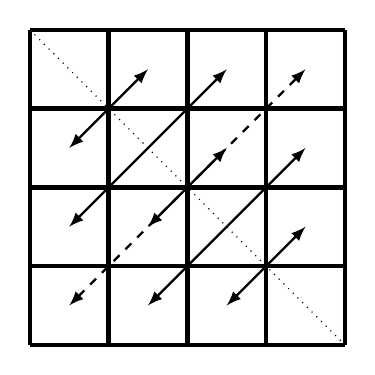
\begin{tikzpicture}
                \draw [latex-latex,thick] (0.5,2.5) -- (1.5,3.5);
                \draw [latex-latex,thick] (0.5,1.5) -- (2.5,3.5);
                \draw [latex-latex,thick,dashed] (0.5,0.5) -- (3.5,3.5);
                \draw [latex-latex,thick] (1.5,1.5) -- (2.5,2.5);
                \draw [latex-latex,thick] (1.5,0.5) -- (3.5,2.5);
                \draw [latex-latex,thick] (2.5,0.5) -- (3.5,1.5);
                \draw [dotted] (0,4) -- (4,0);
                \draw [step=1cm,black,ultra thick] (0,0) grid (4,4);
            \end{tikzpicture}
        \end{center}
        A symmetric matrix is a square matrix that is equal to its transpose. Formally described as:\\[10pt]
        \begin{align*}
            \boxed{\text{A is symmetric} \Longleftrightarrow A = A^T}
        \end{align*}
        Or,
        \begin{align*}
            \boxed{\text{A is symmetric} \Longleftrightarrow \forall~i,j,~~a_{ji} = a_{ij}}
        \end{align*}\\[10pt]
        For example, the following $3\times{3}$ matrix is symmetric:
        \begin{align*}
            A =
            \begin{bmatrix}
                1 & 2 & 3 \\
                2 & 6 & 4 \\
                3 & 4 & 5
            \end{bmatrix}
        \end{align*}
        Since $A = A^T$
    }

    \begin{tabularsection}{Algorithm}
        \begin{algorithmic}[1]
            \State Start
            \State \textbf{read} $A,$ size
            \For {$\forall~i \in \{0,\ldots,\text{size}\}$}
                \For {$\forall~j \in \{0,\ldots,\text{size}\}$}
                    \If{$a_{ij} \neq a_{ji}$}
                        \State \textbf{print} Matrix isn't symmetric
                        \State \textbf{goto} Stop
                    \EndIf
                \EndFor
            \EndFor
            \State \textbf{print} Matrix is symmetric
            \State Stop
        \end{algorithmic}
    \end{tabularsection}

    %------------------------------------------------------------------------------------------------------------------%
\end{document}